%!TeX root = book.tex
%!TEX TS-program = lualatex

\begin{russian}
\chapter[Механика упругого деформирования зернистых композитов со сжатыми сфероидальными зернами]{Механика упругого деформирования зернистых композитов со сжатыми сфероидальными зернами}\chaptermark{Деформирование композитов со сжатыми сфероидальными зернами}

\section[Упругое состояние пространства с несколькими сжатыми сфероидальными полостями]{Упругое состояние пространства с несколькими сжатыми сфероидальными полостями\sectionmark{Упругое состояние пространства со сжатыми сфероидальными полостями}}\sectionmark{Упругое состояние пространства со сжатыми сфероидальными полостями}

Рассмотрим одно(дву)осное растяжение на бесконечности упругого пространства с несколькими сжатыми сфероидальными полостями, расположенными неосесимметрично. Центры полостей находятся в точках $O_j$, а их границы задаются уравнениями

\begin{equation}
\frac{{\rho _j^2}}{{d_{j1}^2}} + \frac{{z_j^2}}{{d_{j2}^2}} = 1,
\label{eq:10:12}
\end{equation}

\noindent где $d_{ij}>0$~--- полуоси сфероидов, $(\rho_j,\varphi_j,z_j)$~--- одинаково направленные цилиндрические системы координат, начала которых совпадают с точками $O_j$. Считается, что полости свободны от нагрузки.

\begin{figure}[h!]
\centering
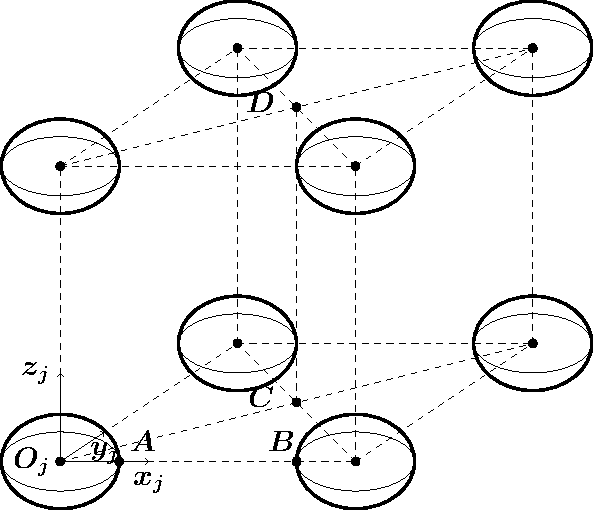
\includegraphics[width=8cm]{oblate-spheroids.pdf}
\caption{Схематическое представление задачи}
\label{f:10:1o}
\end{figure}

Введем вытянутые сфероидальные системы координат $\left( {{{\tilde \xi }_j},{{\tilde \eta }_j},{\varphi _j}} \right)$, совмещенные с цилиндрическими системами. В сфероидальных координатах поверхности полостей задаются уравнениями ${\Gamma _j}:\,{\tilde \xi _j} = {\tilde \xi _{j0}}$, где $\tilde\xi_{j0}$ находят из системы уравнений

\begin{equation}
\left\{ {\begin{array}{*{20}{l}}
{{{\tilde c}_j}{\mathop{\rm ch}\nolimits} {{\tilde \xi }_{j0}} = {d_{j1}},}\\
{{{\tilde c}_j}{\mathop{\rm sh}\nolimits} {{\tilde \xi }_{j0}} = {d_{j2}}.}
\end{array}} \right.
\end{equation}

Для определения НДС в рассматриваемом теле необходимо решить краевую задачу относительно вектора перемещения $\mathbf{U}$, удовлетворяющего уравнению Ламе, граничным условиям на поверхностях $\Gamma_j$

\begin{equation}
{\bf{FU}}{|_{{\Gamma _j}}} = 0\qquad {\kern 1pt} \left( {j = \overline {1,N} } \right)
\label{eq:10:3}
\end{equation}
и условиям на бесконечности~\eqref{eq:9:21}, \eqref{eq:9:22}.

Решение задачи будем искать в виде

\begin{equation}
{\bf{U}} = {\bf{\tilde U}} + {{\bf{U}}_0},
\end{equation}

\begin{equation}
{\bf{\tilde U}} = \sum\limits_{j = 1}^N {\sum\limits_{s = 1}^3 {\sum\limits_{n = 0}^\infty  {\sum\limits_{m =  - n - 1}^{n + 1} {a_{s,n,m}^{(j)}} } } } {\bf{U}}_{s,n,m}^{ + (6)}\left( {{{\tilde \xi }_j},{{\tilde \eta }_j},{\varphi _j}} \right).
\end{equation}

Вспомогательный вектор $\mathbf{U}_0$ описан в~\eqref{eq:9:7}, \eqref{eq:9:8}, $a_{s,n,m}^{(j)}$~--- неизвестные коэффициенты.

Рассмотрим базисные частные решения уравнения Ламе для сжатого сфероида $\Omega _6^ \pm \left\{ {(\xi ,\eta ,\varphi ):{\mkern 1mu} {\kern 1pt} \xi  \mathbin{\lower.3ex\hbox{$\buildrel>\over
{\smash{\scriptstyle<}\vphantom{_x}}$}} {\xi _0}} \right\}$:

\begin{multline}
{\bf{U}}_{s,n,m}^{ \pm (6)}\left( {\tilde \xi ,\tilde \eta ,\varphi } \right) = \\
= \frac{{ - i\tilde c}}{{2n + 1}}{{\bf{D}}_s}\left[ {u_{n - 1,m}^{ \pm (6)}\left( {\tilde \xi ,\tilde \eta ,\varphi } \right) - u_{n + 1,m}^{ \pm (6)}\left( {\tilde \xi ,\tilde \eta ,\varphi } \right)} \right];\qquad {\kern 1pt} s = 1,3;
\label{eq:10:1}
\end{multline}

\begin{equation}
{\bf{U}}_{2,n,m}^{ \pm (6)}\left( {\tilde \xi ,\tilde \eta ,\varphi } \right) = {{\bf{D}}_2}u_{n,m}^{ \pm (6)}\left( {\tilde \xi ,\tilde \eta ,\varphi } \right) - i\tilde c{{\mathop{\rm sh}\nolimits} ^2}{\tilde \xi _0}{{\bf{D}}_1}u_{n \pm 1,m}^{ \pm (6)}\left( {\tilde \xi ,\tilde \eta ,\varphi } \right),
\label{eq:10:2}
\end{equation}
где $n=0,1,\dots$; $|m|\le n+1$; $m,n\in\mathbb{Z}$; $\mathbf{D}_s$ определены в~\eqref{eq:1:41};

\begin{multline}
u_{n,m}^{ \pm (6)}\left( {\tilde \xi ,\tilde \eta ,\varphi } \right) = \\
= \left\{ \begin{array}{l}
Q_n^{ - m}(i{\mathop{\rm sh}\nolimits} \tilde \xi )\\
P_n^{ - m}(i{\mathop{\rm sh}\nolimits} \tilde \xi )
\end{array} \right\}P_n^m(\cos \tilde \eta ){e^{im\varphi }},\qquad {\kern 1pt} n,m \in\mathbb{Z} ,\quad |m| \le n,
\end{multline}
где $P_n^m(x)$, $Q_n^m(x)$~--- функции Лежандра первого и второго родов соответственно.

Приведем координатную форму перемещений~\eqref{eq:10:1}, \eqref{eq:10:2}:

\begin{multline}
{\bf{U}}_{1,n,m}^{ \pm (6)}\left( {\tilde \xi ,\tilde \eta ,\varphi } \right) = \\
= u_{n,m - 1}^{ \pm (6)}\left( {\tilde \xi ,\tilde \eta ,\varphi } \right){{\bf{e}}_{ - 1}} - u_{n,m + 1}^{ \pm (6)}\left( {\tilde \xi ,\tilde \eta ,\varphi } \right){{\bf{e}}_1} - u_{n,m}^{ \pm (6)}\left( {\tilde \xi ,\tilde \eta ,\varphi } \right){{\bf{e}}_0};
\end{multline}

\begin{multline}
{\bf{U}}_{2,n,m}^{ \pm (6)}\left( {\tilde \xi ,\tilde \eta ,\varphi } \right) = i\tilde qu_{1,n,m - 1}^{ \pm (6)}\left( {\tilde \xi ,\tilde \eta ,\varphi } \right){{\bf{e}}_{ - 1}} - i\tilde qu_{1,n,m + 1}^{ \pm (6)}\left( {\tilde \xi ,\tilde \eta ,\varphi } \right){{\bf{e}}_1} - \\
- \left[ {i\tilde qu_{1,n,m}^{ \pm (6)}\left( {\tilde \xi ,\tilde \eta ,\varphi } \right) + \chi u_{n,m}^{ \pm (6)}\left( {\tilde \xi ,\tilde \eta ,\varphi } \right)} \right]{{\bf{e}}_0} + \\
+ i\tilde c\left( {{{\tilde q}^2} - \tilde q_0^2} \right)\nabla u_{n \pm 1,m}^{ \pm (6)}\left( {\tilde \xi ,\tilde \eta ,\varphi } \right);
\end{multline}

\begin{equation}
{\bf{U}}_{3,n,m}^{ \pm (6)}\left( {\tilde \xi ,\tilde \eta ,\varphi } \right) =  - u_{n,m - 1}^{ \pm (6)}\left( {\tilde \xi ,\tilde \eta ,\varphi } \right){{\bf{e}}_{ - 1}} - u_{n,m + 1}^{ \pm (6)}\left( {\tilde \xi ,\tilde \eta ,\varphi } \right){{\bf{e}}_1},
\end{equation}
где $\tilde q = {\mathop{\rm sh}\nolimits} \tilde \xi $, ${\tilde q_0} = {\mathop{\rm sh}\nolimits} {\tilde \xi _0}$;

\begin{equation}
u_{1,n,m}^{ \pm (6)}\left( {\tilde \xi ,\tilde \eta ,\varphi } \right) = \tilde u_{1,n,m}^{ \pm (6)}(\tilde \xi )P_n^m(\cos \tilde \eta ){e^{im\varphi }};
\end{equation}

\begin{equation}
\tilde u_{1,n,m}^{ \pm (6)}(\tilde \xi ) = \left\{ \begin{array}{l}
(n + m + 1)Q_{n + 1}^{ - m}(i\tilde q)\\
 - (n - m)P_{n - 1}^{ - m}(i\tilde q)
\end{array} \right\}.
\end{equation}

В работе~\cite{Nikolaev1998} установлена базисность решений~\eqref{eq:10:1}, \eqref{eq:10:2} в областях $\Omega_6^\pm$.

Справедливы следующие теоремы сложения базисных решений уравнения Ламе для сжатого сфероида:

\begin{multline}
{\bf{U}}_{s,n,m}^{ + (6)}\left( {{{\tilde \xi }_1},{{\tilde \eta }_1},{\varphi _1}} \right) = \\
= \sum\limits_{k = 0}^\infty  {\sum\limits_{l =  - \infty }^\infty  {f_{n,m}^{ + (66)k,l}} } {\bf{U}}_{s,k,l}^{ - (6)}\left( {{{\tilde \xi }_2},{{\tilde \eta }_2},{\varphi _2}} \right),\,s = 1,{\mkern 1mu} {\kern 1pt} 3;
\label{eq:10:4}
\end{multline}

\begin{multline}
{\bf{U}}_{2,n,m}^{ + (6)}\left( {{{\tilde \xi }_1},{{\tilde \eta }_1},{\varphi _1}} \right) = \sum\limits_{k = 0}^\infty  {\sum\limits_{l =  - \infty }^\infty  {\left[ {f_{n,m}^{ + (66)k,l}} \right.} } {\bf{U}}_{2,k,l}^{ - (6)}\left( {{{\tilde \xi }_2},{{\tilde \eta }_2},{\varphi _2}} \right) + \\
\left. { + \tilde f_{n,m}^{ + (66)k,l}{\bf{U}}_{1,k,l}^{ - (6)}\left( {{{\tilde \xi }_2},{{\tilde \eta }_2},{\varphi _2}} \right)} \right];
\label{eq:10:5}
\end{multline}

\begin{equation}
f_{n,m}^{ + (66)k,l} = \sum\limits_{j = n}^\infty  {g_{n,m}^{ + (64)j}} ({\tilde c_1})f_{j,m}^{(46)k,l}({\tilde c_2});
\end{equation}

\begin{multline}
g_{n,m}^{ + (64)j}({\tilde c_1}) = \\
= {( - 1)^m}\sqrt \pi  {( - i)^{j + 1}}{\left( {\frac{{{{\tilde c}_1}}}{2}} \right)^{j + 1}}\frac{{{\varepsilon _{jn}}}}{{\Gamma \left( {\frac{{j - n}}{2} + 1} \right)\Gamma \left( {\frac{{j + n}}{2} + \frac{3}{2}} \right)}};
\end{multline}

\begin{multline}
f_{j,m}^{(46)k,l}({\tilde c_2}) = \\
= \sum\limits_{p = 0}^\infty  {{{( - 1)}^{p + l}}} \sqrt \pi  {( - i)^p}{\left( {\frac{{{{\tilde c}_2}}}{2}} \right)^p}\frac{{{\varepsilon _{pk}}\left( {k + \frac{1}{2}} \right)u_{j + p,m - l}^{ + (4)}\left( {{r_{12}},{\theta _{12}},{\varphi _{12}}} \right)}}{{\Gamma \left( {\frac{{p - k}}{2} + 1} \right)\Gamma \left( {\frac{{p + k}}{2} + \frac{3}{2}} \right)}};
\end{multline}

\begin{multline}
\tilde f_{n,m}^{ + (66)k,l} = \sum\limits_{j = n}^\infty  {\left[ {i{{\tilde c}_2}\tilde q_{20}^2\frac{{2k + 1}}{{2k + 3}}} \right.} g_{n,m}^{ + (64)j}f_{j + 1,m}^{(46)k + 1,l} + {z_{12}}g_{n,m}^{ + (64)j}f_{j + 1,m}^{(46)k,l} - \\
\left. {\frac{{}}{{}}i{{\tilde c}_1}\tilde q_{10}^2g_{n + 1,m}^{ + (64)j - 1}f_{j,m}^{(46)k,l}} \right];
\end{multline}

\begin{multline}
{\bf{U}}_{s,n,m}^{ + (6)}\left( {{{\tilde \xi }_2},{{\tilde \eta }_2},{\varphi _2}} \right) = \\
= \sum\limits_{k = 0}^\infty  {\sum\limits_{l =  - \infty }^\infty  {f_{n,m}^{ - (66)k,l}} } {\bf{U}}_{s,k,l}^{ - (6)}\left( {{{\tilde \xi }_1},{{\tilde \eta }_1},{\varphi _1}} \right),\,s = 1,{\mkern 1mu} {\kern 1pt} 3;
\label{eq:10:6}
\end{multline}

\begin{multline}
{\bf{U}}_{2,n,m}^{ + (6)}\left( {{{\tilde \xi }_2},{{\tilde \eta }_2},{\varphi _2}} \right) = \sum\limits_{k = 0}^\infty  {\sum\limits_{l =  - \infty }^\infty  {\left[ {f_{n,m}^{ - (66)k,l}} \right.} } {\bf{U}}_{2,k,l}^{ - (6)}\left( {{{\tilde \xi }_1},{{\tilde \eta }_1},{\varphi _1}} \right) + \\
\left. { + \tilde f_{n,m}^{ - (66)k,l}{\bf{U}}_{1,k,l}^{ - (6)}\left( {{{\tilde \xi }_1},{{\tilde \eta }_1},{\varphi _1}} \right)} \right];
\label{eq:10:7}
\end{multline}

\begin{equation}
f_{n,m}^{ - (66)k,l} = \sum\limits_{j = k}^\infty  {f_{n,m}^{(64)j,l}({{\tilde c}_2})g_{j,l}^{ - (46)k}} ({\tilde c_1});
\end{equation}

\begin{multline}
f_{n,m}^{(64)j,l}({\tilde c_2}) = \\
= \sum\limits_{p = 0}^\infty  {{{( - 1)}^{p + l + m}}} \sqrt \pi  {( - i)^{p + 1}}{\left( {\frac{{{{\tilde c}_2}}}{2}} \right)^{p + 1}}\frac{{{\varepsilon _{pn}}u_{p + j,m - l}^{ + (4)}\left( {{r_{12}},{\theta _{12}},{\varphi _{12}}} \right)}}{{\Gamma \left( {\frac{{p - n}}{2} + 1} \right)\Gamma \left( {\frac{{p + n}}{2} + \frac{3}{2}} \right)}};
\end{multline}

\begin{multline}
\tilde f_{n,m}^{ - (66)k,l} = \sum\limits_{j = k}^\infty\bigg[i{{\tilde c}_2}\tilde q_{20}^2f_{n + 1,m}^{(64)j + 1,l}({{\tilde c}_2})g_{j,l}^{ - (46)k}({{\tilde c}_1}) + \\
+ {z_{12}}f_{n,m}^{(64)j + 1,l}({{\tilde c}_2})g_{j,l}^{ - (46)k}({{\tilde c}_1}) - \frac{{}}{{}}i{{\tilde c}_1}\tilde q_{10}^2\frac{{2k + 1}}{{2k + 3}}f_{n,m}^{(64)j,l}({{\tilde c}_2})g_{j - 1,l}^{ - (46)k + 1}({{\tilde c}_1}) \bigg].
\end{multline}

Приведем формулы для напряжений, отвечающих базисным перемещениям ${\bf{U}}_{s,n,m}^{ \pm (6)}\left( {{{\tilde \xi }_j},{{\tilde \eta }_j},{\varphi _j}} \right)$ на поверхностях $\Gamma_j$ ($\mathbf{n}_j=\mathbf{e}_{\tilde\xi_j}$~--- нормаль к поверхности $\Gamma_j$):

\begin{multline}
{\bf{FU}}_{1,n,m}^{ \pm (6)}\left( {{{\tilde \xi }_j},{{\tilde \eta }_j},{\varphi _j}} \right) = 2G\frac{{{{\tilde H}_j}}}{{{{\tilde c}_j}}}\left[ {\frac{\partial }{{\partial {{\tilde \xi }_j}}}u_{n,m - 1}^{ \pm (6)}\left( {{{\tilde \xi }_j},{{\tilde \eta }_j},{\varphi _j}} \right){{\bf{e}}_{ - 1}} - } \right.\\
\left. { - \frac{\partial }{{\partial {{\tilde \xi }_j}}}u_{n,m + 1}^{ \pm (6)}\left( {{{\tilde \xi }_j},{{\tilde \eta }_j},{\varphi _j}} \right){{\bf{e}}_1} - \frac{\partial }{{\partial {{\tilde \xi }_j}}}u_{n,m}^{ \pm (6)}\left( {{{\tilde \xi }_j},{{\tilde \eta }_j},{\varphi _j}} \right){{\bf{e}}_0}} \right];
\label{eq:10:25o}
\end{multline}

\begin{multline}
{\bf{FU}}_{2,n,m}^{ \pm (6)}\left( {{{\tilde \xi }_j},{{\tilde \eta }_j},{\varphi _j}} \right) = 2G\frac{{{{\tilde H}_j}}}{{{{\tilde c}_j}}}\left\{ {\left[ { - \bar q_j^2\frac{\partial }{{\partial {{\tilde \xi }_j}}}\left( {\frac{{u_{1,n,m - 1}^{ \pm (6)}}}{{{{\bar q}_j}}}} \right) - 2\sigma u_{2,n,m}^{ \pm (6)}} \right]{{\bf{e}}_{ - 1}} - } \right.\\
- \left[ { - \bar q_j^2\frac{\partial }{{\partial {{\tilde \xi }_j}}}\left( {\frac{{u_{1,n,m + 1}^{ \pm (6)}}}{{{{\bar q}_j}}}} \right) - 2\sigma u_{3,n,m}^{ \pm (6)}} \right]{{\bf{e}}_1} - \left[ { - \tilde q_j^2\frac{\partial }{{\partial {{\tilde \xi }_j}}}\left( {\frac{{u_{1,n,m}^{ \pm (6)}}}{{{{\bar q}_j}}}} \right) + } \right.\\
\left. { + \left. {(1 - 2\sigma )\frac{\partial }{{\partial {{\tilde \xi }_j}}}u_{n,m}^{ \pm (6)}} \right]{{\bf{e}}_0}} \right\};
\label{eq:10:26o}
\end{multline}

\begin{multline}
{\bf{FU}}_{3,n,m}^{ \pm (6)}\left( {{\tilde \xi _j},{\eta _j},{\varphi _j}} \right) = 2G\frac{{{{\tilde H}_j}}}{{{{\tilde c}_j}}}\left\{ { - \left[ {\frac{\partial }{{\partial {{\tilde \xi }_j}}}u_{n,m - 1}^{ \pm (6)} - \frac{1}{2}u_{2,n,m}^{ \pm (6)}} \right]{{\bf{e}}_{ - 1}} - } \right.\\
\left. { - \left[ {\frac{\partial }{{\partial {{\tilde \xi }_j}}}u_{n,m + 1}^{ \pm (6)} - \frac{1}{2}u_{3,n,m}^{ \pm (6)}} \right]{{\bf{e}}_1} + \frac{m}{2}\frac{{{{\bar q}_j}}}{{{q_j}}}u_{n,m}^{ \pm (6)}{{\bf{e}}_0}} \right\},
\label{eq:10:27o}
\end{multline}

где ${\tilde H_j} = {\left( {\bar q_j^2 + {{\cos }^2}{{\tilde \eta }_j}} \right)^{ - \frac{1}{2}}}$;
$$
u_{1,n,m}^{ \pm (6)}\left( {{{\tilde \xi }_j},{{\tilde \eta }_j},{\varphi _j}} \right) = \tilde u_{1,n,m}^{ \pm (6)}({\tilde \xi _j})P_n^m(\cos {\tilde \eta _j}){e^{im{\varphi _j}}};
$$
$$
u_{2,n,m}^{ \pm (6)}\left( {{{\tilde \xi }_j},{{\tilde \eta }_j},{\varphi _j}} \right) = \tilde u_{2,n,m}^{ \pm (6)}({\tilde \xi _j})P_n^{m - 1}(\cos {\tilde \eta _j}){e^{i(m - 1){\varphi _j}}};
$$
$$
u_{3,n,m}^{ \pm (6)}\left( {{{\tilde \xi }_j},{{\tilde \eta }_j},{\varphi _j}} \right) = \tilde u_{n,m}^{ \pm (6)}({\tilde \xi _j})P_n^{m + 1}(\cos {\tilde \eta _j}){e^{i(m + 1){\varphi _j}}};
$$
$$
\tilde u_{n,m}^{ \pm (6)}(\xi ) = \left\{ \begin{array}{l}
Q_n^{ - m}(i\bar q)\\
P_n^{ - m}(i\bar q)
\end{array} \right\};\qquad {\kern 1pt} \tilde u_{1,n,m}^{ \pm (6)}(\tilde \xi ) = \left\{ \begin{array}{l}
(n + m + 1)Q_{n + 1}^{ - m}(i\bar q)\\
 - (n - m)P_{n - 1}^{ - m}(i\bar q)
\end{array} \right\};
$$
$$
\tilde u_{2,n,m}^{ \pm (6)}(\tilde \xi ) = (n + m)(n - m + 1)\tilde u_{n,m}^{ \pm (6)}(\tilde \xi ),\qquad {\kern 1pt} q = {\mathop{\rm ch}\nolimits} \tilde \xi ,\quad \bar q = {\mathop{\rm sh}\nolimits} \tilde\xi.
$$

Относительно перемещения $\mathbf{\tilde U}$ граничные условия~\eqref{eq:10:3} можно записать так:

\begin{equation}
{\bf{F\tilde U}}{|_{{\Gamma _j}}} =  - {\bf{F}}{{\bf{U}}_0}{|_{{\Gamma _j}}}.
\end{equation}

На бесконечности вектор $\mathbf{F\tilde U}$ подчиняется условиям~\eqref{eq:9:21}, \eqref{eq:9:22}. Заметим, что вектор усилий ${\bf{F}}{{\bf{U}}_0}{|_{{\Gamma _j}}}$ для каждого типа растяжений упругого пространства находят по формулам $(\mathbf{n}_j=\mathbf{e}_{\tilde\xi_j})$

\begin{equation}
{\bf{F}}{{\bf{U}}_0}{|_{{\Gamma _j}}} = T{\tilde H_j}{\mathop{\rm ch}\nolimits} {\tilde \xi _{j0}}{P_1}(\cos {\tilde \eta _j}){{\bf{e}}_z}\quad\text{(одноосное растяжение)},
\end{equation}

\begin{equation}
{\bf{F}}{{\bf{U}}_0}{|_{{\Gamma _j}}} =  - T{\tilde H_j}{\mathop{\rm sh}\nolimits} {\tilde \xi _{j0}}P_1^{(1)}(\cos {\tilde \eta _j}){{\bf{e}}_{{\rho _j}}}\quad\text{(двуосное растяжение)}.
\end{equation}

Используя теоремы сложения~\eqref{eq:10:4}, \eqref{eq:10:5} и \eqref{eq:10:6}, \eqref{eq:10:7}, перемещение $\mathbf{\tilde U}$ можно записать в системе координат с началом в точке $O_j$:

\begin{multline}
{\bf{\tilde U}} = \sum\limits_{s = 1}^3 {\sum\limits_{n = 0}^\infty  {\sum\limits_{m =  - n - 1}^{n + 1} {a_{s,n,m}^{(j)}} } } {\bf{U}}_{s,n,m}^{ + (6)}\left( {{{\tilde \xi }_j},{{\tilde \eta }_j},{\varphi _j}} \right) + \\
+ \sum\limits_{n = 0}^\infty  {\sum\limits_{m =  - n - 1}^{n + 1} {\left\{ {{\bf{U}}_{1,n,m}^{ - (6)}\left( {{{\tilde \xi }_j},{{\tilde \eta }_j},{\varphi _j}} \right)\sum\limits_{\alpha  \ne j} {\sum\limits_{k = 0}^\infty  {\sum\limits_{l =  - k - 1}^{k + 1} {\left[ {a_{1,k,l}^{(\alpha )}f_{k,l,j,\alpha }^{ - (66)n,m} + } \right.} } } } \right.} } \\
\left. { + a_{2k,l}^{(\alpha )}\tilde f_{k,l,j,\alpha }^{ - (66)n,m}} \right] + {\bf{U}}_{2,n,m}^{ - (6)}\left( {{{\tilde \xi }_j},{{\tilde \eta }_j},{\varphi _j}} \right)\sum\limits_{\alpha  \ne j} {\sum\limits_{k = 0}^\infty  {\sum\limits_{l =  - k - 1}^{k + 1} {a_{2,k,l}^{(\alpha )}} } \tilde f_{k,l,j,\alpha }^{ - (66)n,m} + } \\
\left. { + {\bf{U}}_{3,n,m}^{ - (6)}\left( {{{\tilde \xi }_j},{{\tilde \eta }_j},{\varphi _j}} \right)\sum\limits_{\alpha  \ne j} {\sum\limits_{k = 0}^\infty  {\sum\limits_{l =  - k - 1}^{k + 1} {a_{3,k,l}^{(\alpha )}} } f_{k,l,j,\alpha }^{ - (66)n,m}} } \right\}.
\label{eq:10:8}
\end{multline}

После перехода в формулах~\eqref{eq:10:8} к напряжениям и удовлетворения граничных условий относительно неизвестных $a_{s,n,m}^{(j)}$ получаем бесконечную систему линейных алгебраических уравнений:

\begin{multline}
\sum\limits_{s = 1}^3 {a_{s,n,m}^{(1)}} \tilde W_{s,n,m}^{ + (k)}({\tilde \xi _{10}}) + \tilde W_{1,n,m}^{ - (k)}({\tilde \xi _{10}})\sum\limits_{k = 0}^\infty  {\sum\limits_{l =  - k - 1}^{k + 1} {\left[ {a_{1,k,l}^{(2)}f_{k,l}^{ - (66)n,m} + } \right.} } \\
\left. { + a_{2,k,l}^{(2)}\tilde f_{k,l}^{ - (66)n,m}} \right] + \tilde W_{2,n,m}^{ - (k)}({\tilde \xi _{10}})\sum\limits_{k = 0}^\infty  {\sum\limits_{l =  - k - 1}^{k + 1} {a_{2,k,l}^{(2)}} } f_{k,l}^{ - (66)n,m} + \\
+ \tilde W_{3,n,m}^{ - (k)}({\tilde \xi _{10}})\sum\limits_{k = 0}^\infty  {\sum\limits_{l =  - k - 1}^{k + 1} {a_{3,k,l}^{(2)}} } f_{k,l}^{ - (66)n,m} = \tilde W_{n,m}^{(k)j};
\end{multline}
$$
n,m \in\mathbb{Z}:\quad n \ge 0,\quad |m| \le n + 1,\quad k =  - 1,{\mkern 1mu} {\kern 1pt} 0,{\mkern 1mu} {\kern 1pt} 1;
$$

\begin{equation}
\tilde W_{1,n,m}^{ \pm ( - 1)}(\tilde \xi ) = \frac{\partial }{{\partial \tilde \xi }}\tilde u_{n,m - 1}^{ \pm (6)}(\tilde \xi ),\quad \tilde W_{1,n,m}^{ \pm (1)} =  - \frac{\partial }{{\partial \tilde \xi }}\tilde u_{n,m + 1}^{ \pm (6)}(\tilde \xi );
\end{equation}

\begin{equation}
\tilde W_{1,n,m}^{ \pm (0)}(\tilde \xi ) =  - \frac{\partial }{{\partial \tilde \xi }}\tilde u_{n,m}^{ \pm (6)}(\tilde \xi );
\end{equation}
\begin{equation}
\tilde W_{2,n,m}^{ \pm ( - 1)}(\tilde \xi ) = i{\bar q^2}\frac{\partial }{{\partial \tilde \xi }}\left[ {\frac{{\tilde u_{1,n,m - 1}^{ \pm (6)}(\tilde \xi )}}{{\bar q}}} \right] - 2\sigma \tilde u_{2,n,m}^{ \pm (6)}(\tilde \xi );
\end{equation}

\begin{equation}
\tilde W_{2,n,m}^{ \pm (1)}(\tilde \xi ) =  - i{\bar q^2}\frac{\partial }{{\partial \tilde \xi }}\left[ {\frac{{u_{1,n,m + 1}^{ \pm (6)}(\tilde \xi )}}{{\bar q}}} \right] + 2\sigma \tilde u_{n,m}^{ \pm (6)}(\tilde \xi );
\end{equation}

\begin{equation}
\tilde W_{2,n,m}^{ \pm (0)}(\tilde \xi ) =  - i{\bar q^2}\frac{\partial }{{\partial \tilde \xi }}\left[ {\frac{{\tilde u_{1,n,m}^{ \pm (6)}(\tilde \xi )}}{{\bar q}}} \right] - (1 - 2\sigma )\frac{\partial }{{\partial \tilde \xi }}\tilde u_{n,m}^{ \pm (6)}(\tilde \xi );
\end{equation}

\begin{equation}
\tilde W_{3,n,m}^{ \pm ( - 1)}(\tilde \xi ) =  - \frac{\partial }{{\partial \tilde \xi }}\tilde u_{n,m - 1}^{ \pm (6)}(\tilde \xi ) + \frac{1}{2}\tilde u_{2,n,m}^{ \pm (6)}(\tilde \xi );
\end{equation}

\begin{equation}
\tilde W_{3,n,m}^{ \pm (1)}(\tilde \xi ) =  - \frac{\partial }{{\partial \tilde \xi }}\tilde u_{n,m + 1}^{ \pm (6)}(\tilde \xi ) + \frac{1}{2}\tilde u_{n,m}^{ \pm (6)}(\tilde \xi );
\end{equation}
\begin{equation}
\tilde W_{3,n,m}^{ \pm (0)}(\tilde \xi ) = \frac{m}{2}\frac{{\bar q}}{q}\tilde u_{n,m}^{ \pm (6)}(\tilde \xi );
\end{equation}

\begin{equation}
\tilde W_{n,m}^{(k)j} = \left\{ \begin{array}{l}
 - \dfrac{T}{{2G}}{{\tilde c}_j}{\mathop{\rm ch}\nolimits} {{\tilde \xi }_{j0}}{\delta _{n1}}{\delta _{m0}}\quad\text{(одноосное растяжение)},\\ \\
\dfrac{T}{{2G}}{{\tilde c}_j}{\mathop{\rm sh}\nolimits} {{\tilde \xi }_{j0}}{\delta _{n1}}{\delta _{m0}}\quad\text{(двуосное растяжение)}.
\end{array} \right.
\end{equation}

\subsection{Анализ численных результатов для пространства со сжатыми сфероидальными полостями при одноосном и двуосном растяжениях}

\sidefig[t](99mm){
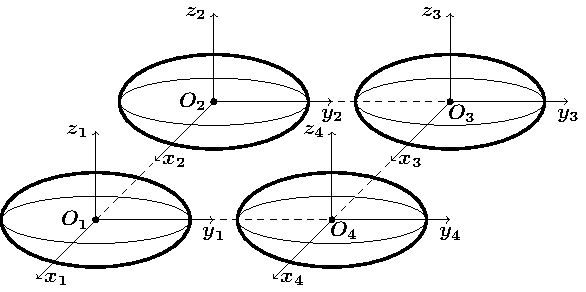
\includegraphics[width=10cm]{cartesian-oblate-spheroids-4.pdf}
\caption{Четыре сжатые сфероидальные полости}
\label{f:10:1}
}{Рассмотрим одноосное и двуосное растяжения упругого пространства с четырьмя сжатыми сфероидальными полостями. Полости расположены в вершинах квадрата (рис.~\ref{f:10:1}). Считается, что полости свободны от нагрузки.

При численном анализе полагаем коэффициент Пуассона материала упругого} пространства $\sigma=0.38$, полости считаем одного размера, отношение полуосей сфероидов~--- $d_2/d_1=0.5$. Разрешающую систему уравнений численно решаем методом редукции. На основании полученных решений находим нормальные напряжения на площадках, параллельных координатным плоскостям.

На рис.~\ref{f:10:2}~--- \ref{f:10:4} приведены напряжения $\sigma_x/T$, $\sigma_y/T$ и $\sigma_z/T$ на линии $O_1O_4$ (см.~рис.~\ref{f:10:1}) вне полостей при одноосном растяжении в зависимости от относительного расстояния $a/d_1$ между полостями.

Областью концентрации напряжений $\sigma_y/T$ и $\sigma_z/T$ является граница полостей, в то время как напряжения $\sigma_x/T$ достигают максимальных значений в окрестности середины отрезка $O_1O_4$. Для всех случаев характерен рост напряжений с приближением полостей друг к другу.

На рис.~\ref{f:10:5}~--- \ref{f:10:7} приведены напряжения $\sigma_x/T$, $\sigma_y/T$ и $\sigma_z/T$ на линии $O_1O_4$ (рис.~\ref{f:10:1}) вне полостей при двуосном растяжении в зависимости от относительного расстояния $a/d_1$ между полостями.

\begin{figure}[h!]
\centering\footnotesize
\parbox[b]{7.5cm}{\centering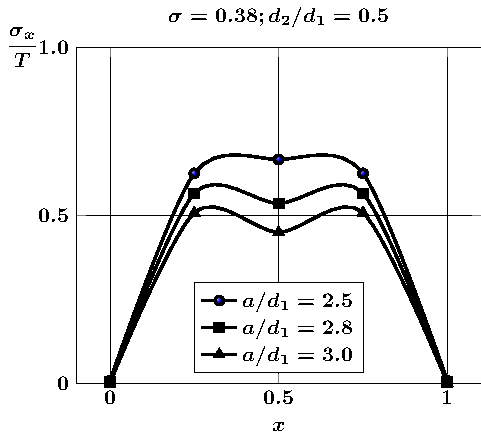
\includegraphics[width=7.6cm]{cav4-oblate-a-d50-t1-sig_x.pdf}
\caption{Напряжения $\sigma_x/T$ на линии $O_1O_4$ в зависимости от относительного расстояния между полостями при одноосном растяжении
\label{f:10:2}}}\hfil\hfil
\parbox[b]{7.5cm}{\centering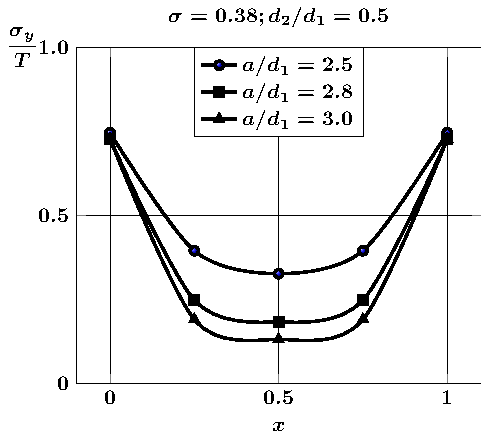
\includegraphics[width=7.6cm]{cav4-oblate-a-d50-t1-sig_y.pdf}
\caption{Напряжения $\sigma_y/T$ на линии $O_1O_4$ в зависимости от относительного расстояния между полостями при одноосном растяжении
\label{f:10:3}}}
\end{figure}

\begin{figure}[h!]
\centering\footnotesize
\parbox[b]{7.5cm}{\centering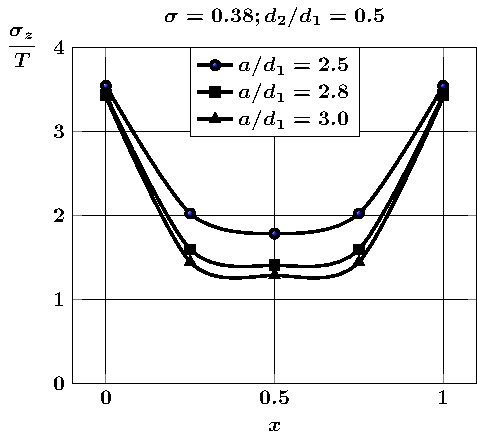
\includegraphics[width=7.6cm]{cav4-oblate-a-d50-t1-sig_z.pdf}
\caption{Напряжения $\sigma_z/T$ на линии $O_1O_4$ в зависимости от относительного расстояния между полостями при одноосном растяжении
\label{f:10:4}}}\hfil\hfil
\parbox[b]{7.5cm}{\centering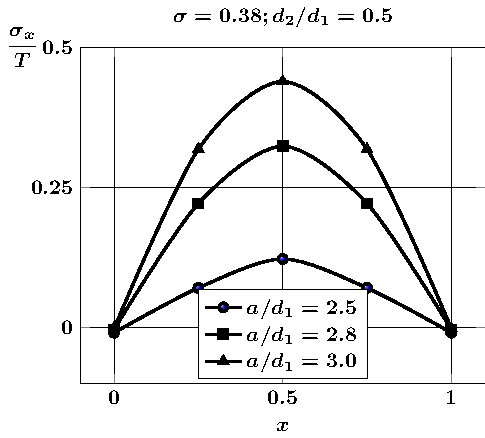
\includegraphics[width=7.6cm]{cav4-oblate-a-d50-t2-sig_x.pdf}
\caption{Напряжения $\sigma_x/T$ на линии $O_1O_4$ в зависимости от относительного расстояния между полостями при двуосном растяжении
\label{f:10:5}}}
\end{figure}

Напряжения $\sigma_x/T$ убывают с приближением полостей друг к другу. Напряжения $\sigma_y/T$ растут с приближением полостей и для случая $a/d_1=2.5$ практически постоянны на всем рассматриваемом отрезке. Областью концентрации напряжений $\sigma_z/T$ являются границы полостей, причем с удалением полостей друг от друга напряжения $\sigma_z/T$ растут по модулю, оставаясь вблизи полостей сжимающими.

На рис.~\ref{f:10:8}~--- \ref{f:10:10} представлены напряжения $\sigma_x/T$, $\sigma_y/T$ и $\sigma_z/T$ на линии $O_1O_4$ вне полостей при одноосном растяжении в зависимости от отношения вертикальной полуоси сфероида к его горизонтальной полуоси при $a/d_1=3.5$.

\begin{figure}[h!]
\centering\footnotesize
\parbox[b]{7.5cm}{\centering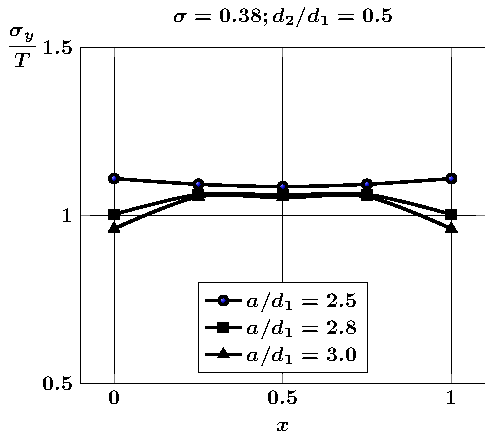
\includegraphics[width=7.6cm]{cav4-oblate-a-d50-t2-sig_y.pdf}
\caption{Напряжения $\sigma_y/T$ на линии $O_1O_4$ в зависимости от относительного расстояния между полостями при двуосном растяжении
\label{f:10:6}}}\hfil\hfil
\parbox[b]{7.5cm}{\centering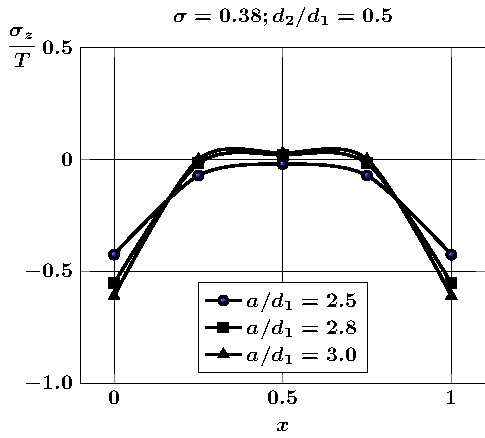
\includegraphics[width=7.6cm]{cav4-oblate-a-d50-t2-sig_z.pdf}
\caption{Напряжения $\sigma_z/T$ на линии $O_1O_4$ в зависимости от относительного расстояния между полостями при двуосном растяжении
\label{f:10:7}}}
\end{figure}

\begin{figure}[h!]
\centering\footnotesize
\parbox[b]{7.5cm}{\centering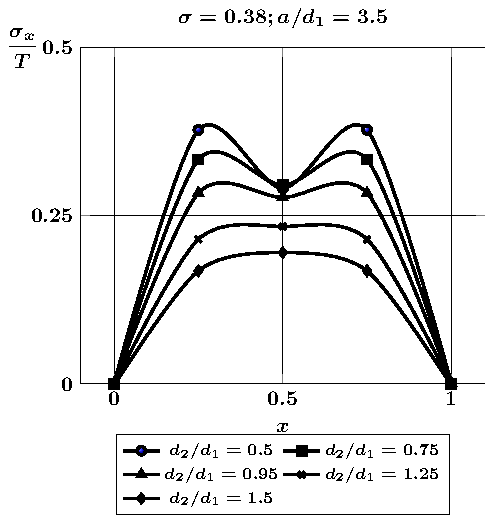
\includegraphics[width=7.6cm]{cav4-prolate-oblate-a35-t1-sig_x.pdf}
\caption{Напряжения $\sigma_x/T$ на линии $O_1O_4$ в зависимости от отношения полуосей сфероида при одноосном растяжении
\label{f:10:8}}}\hfil\hfil
\parbox[b]{7.5cm}{\centering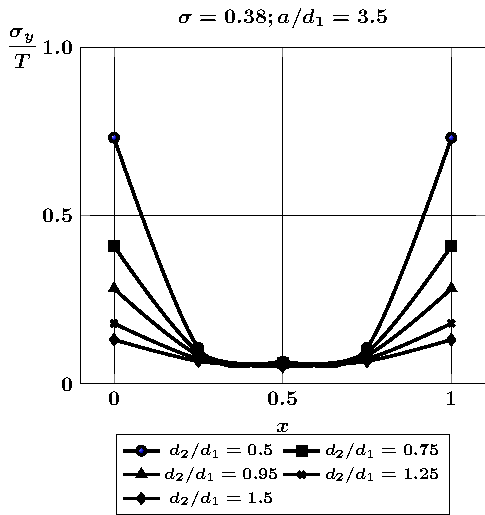
\includegraphics[width=7.6cm]{cav4-prolate-oblate-a35-t1-sig_y.pdf}
\caption{Напряжения $\sigma_y/T$ на линии $O_1O_4$ в зависимости от отношения полуосей сфероида при одноосном растяжении
\label{f:10:9}}}
\end{figure}

\begin{figure}[h!]
\centering\footnotesize
\parbox[b]{7.5cm}{\centering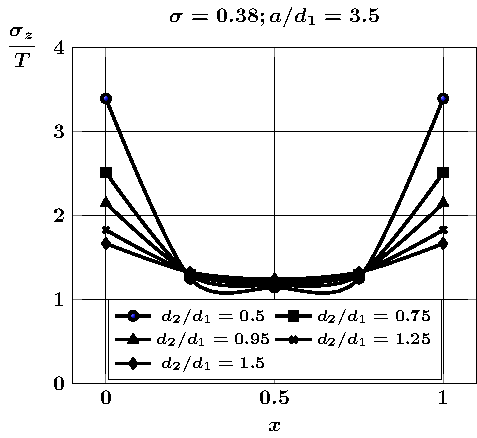
\includegraphics[width=7.6cm]{cav4-prolate-oblate-a35-t1-sig_z.pdf}
\caption{Напряжения $\sigma_z/T$ на линии $O_1O_4$ в зависимости от отношения полуосей сфероида при одноосном растяжении
\label{f:10:10}}}\hfil\hfil
\parbox[b]{7.5cm}{\centering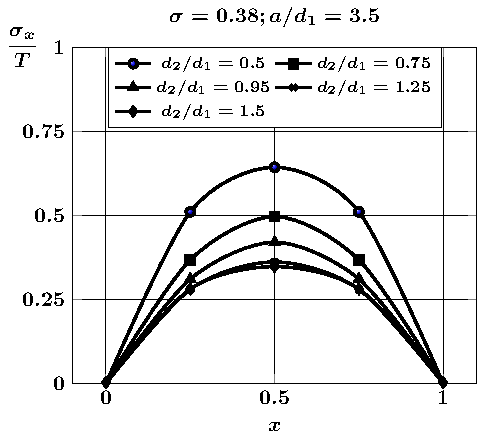
\includegraphics[width=7.6cm]{cav4-prolate-oblate-a35-t2-sig_x.pdf}
\caption{Напряжения $\sigma_x/T$ на линии $O_1O_4$ в зависимости от отношения полуосей сфероида при двуосном растяжении
\label{f:10:11}}}
\end{figure}

Наибольшие значения напряжений $\sigma_x/T$ наблюдаются при наименьшем отношении $d_2/d_1$. Для случая сжатых сфероидальных полостей присутствует ярко выраженная двухмодальность кривых в распределении напряжений.

Для напряжений $\sigma_y/T$ в середине рассматриваемого отрезка имеется область, в которой напряжения практически не зависят от отношения $d_2/d_1$, в то время как вблизи границ полостей есть область концентрации напряжений, в которой напряжения растут при уменьшении $d_2/d_1$. Похожая ситуация наблюдается и для напряжений $\sigma_z/T$.

Напряжения $\sigma_x/T$ концентрируются в середине отрезка и возрастают с уменьшением $d_2/d_1$. Для напряжений $\sigma_y/T$ характерно изменение направления выпуклости кривых при переходе от вытянутых сфероидальных полостей к сжатым сфероидальным. Для напряжений $\sigma_z/T$ наблюдается концентрация у границ полостей, при этом они растут по модулю с уменьшением отношения $d_2/d_1$.

На рис.~\ref{f:10:11}~--- \ref{f:10:13} приведены напряжения $\sigma_x/T$, $\sigma_y/T$ и $\sigma_z/T$ на линии $O_1O_4$ вне полостей при двуосном растяжении в зависимости от отношения вертикальной полуоси сфероида к его горизонтальной полуоси при $a/d_1=\\=3.5$.

По результатам проведенных вычислений можно сделать следующие выводы:
\begin{enumerate}
\item В случае одноосного растяжения наибольшей концентрацией (в 3.5 раза) обладают напряжения $\sigma_z/T$ на границах полостей, при этом коэффициент концентрации практически не зависит от взаимной близости полостей.
\item С уменьшением вертикальной полуоси сфероидов $d_2$ (переход от вытянутых сфероидов к сжатым) при фиксированном расстоянии между полостями все напряжения в области их концентрации растут при одноосном растяжении.
\item В случае двуосного растяжения наибольшей концентрацией (в 1.5 раза) обладают напряжения $\sigma_y/T$ на границах полостей, при этом коэффициент концентрации растет с ростом $d_2$ при фиксированном расстоянии между полостями.
\end{enumerate}

\begin{figure}[h!]
\centering\footnotesize
\parbox[b]{7.5cm}{\centering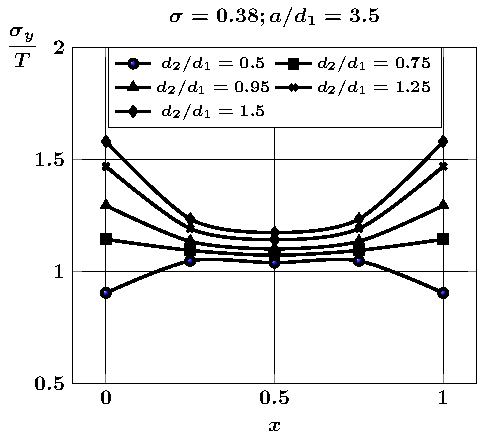
\includegraphics[width=7.6cm]{cav4-prolate-oblate-a35-t2-sig_y.pdf}
\caption{Напряжения $\sigma_y/T$ на линии $O_1O_4$ в зависимости от отношения полуосей сфероида при двуосном растяжении
\label{f:10:12}}}\hfil\hfil
\parbox[b]{7.5cm}{\centering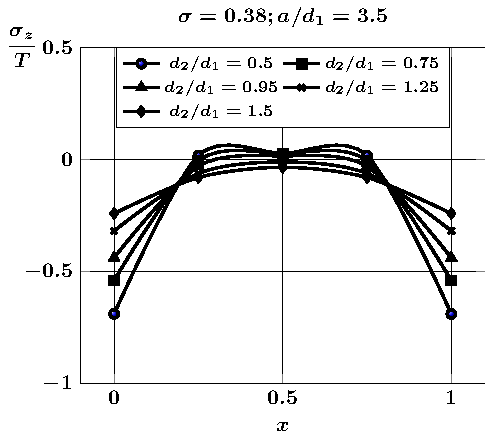
\includegraphics[width=7.6cm]{cav4-prolate-oblate-a35-t2-sig_z.pdf}
\caption{Напряжения $\sigma_z/T$ на линии $O_1O_4$ в зависимости от отношения полуосей сфероида при двуосном растяжении
\label{f:10:13}}}
\end{figure}

\section[Упругое состояние пространства с несколькими сжатыми сфероидальными включениями]{Упругое состояние пространства с несколькими сжатыми сфероидальными включениями\sectionmark{Упругое состояние пространства со сжатыми сфероидальными включениями}}\sectionmark{Упругое состояние пространства со сжатыми сфероидальными включениями}

Рассмотрим постановку задачи предыдущего параграфа в случае, когда сферические полости заполнены упругими материалами с механическими характеристиками ($\sigma_j$, $G_j$). Упругие постоянные матрицы будем считать равными ($\sigma$, $G$).

Граничные условия~\eqref{eq:10:3} нужно заменить условиями сопряжения полей перемещений и напряжений на поверхностях $\Gamma_j$. Для того, чтобы их записать, представим вектор перемещений в упругом пространстве в виде

\begin{equation}
{\bf{U}} = \left\{ {\begin{array}{*{20}{l}}
{{\bf{\tilde U}}_j^ - ,\quad \left( {x,y,z} \right) \in {\Omega _j},}\\
{{{{\bf{\tilde U}}}^ + } + {{\bf{U}}_0},\quad \left( {x,y,z} \right) \in\mathbb{R}^3\backslash {\Omega _j},}
\end{array}} \right.
\label{eq:10:11}
\end{equation}
где ${\Omega _j} = \left\{ {\left( {{{\tilde \xi }_j},{{\tilde \eta }_j},{\varphi _j}} \right):\,{{\tilde \xi }_j} < {{\tilde \xi }_{j0}}} \right\}$. Тогда условия сопряжения принимают следующий вид:

\begin{equation}
\left( {{{{\bf{\tilde U}}}^ + } + {{\bf{U}}_0}} \right){|_{{\Gamma _j}}} = {\bf{\tilde U}}_j^ - {|_{{\Gamma _j}}};
\label{eq:10:9}
\end{equation}

\begin{equation}
\left( {{\bf{F\tilde U}} + {\bf{F}}{{\bf{U}}_0}} \right){|_{{\Gamma _j}}} = {\bf{F}}{{\bf{\tilde U}}_j}{|_{{\Gamma _j}}},\qquad {\kern 1pt} j = \overline {1,N}.
\label{eq:10:10}
\end{equation}

Вектор-функции $\mathbf{\tilde U}^+$, $\mathbf{\tilde U}_j^-$ будем искать в виде

\begin{equation}
{{\bf{\tilde U}}^ + } = \mathop \sum \limits_{j = 1}^N \sum\limits_{s = 1}^3 {\sum\limits_{n = 0}^\infty  {\sum\limits_{m =  - n - 1}^{n + 1} {a_{s,n,m}^{(j)}} } } {\bf{U}}_{s,n,m}^{ + (6)}\left( {{{\tilde \xi }_j},{{\tilde \eta }_j},{\varphi _j}} \right),
\end{equation}

\begin{equation}
{\bf{\tilde U}}_j^ -  = \sum\limits_{s = 1}^3 {\sum\limits_{n = 0}^\infty  {\sum\limits_{m =  - n - 1}^{n + 1} {b_{s,n,m}^{(j)}} } } {\bf{U}}_{s,n,m}^{ - (6)}\left( {{{\tilde \xi }_j},{{\tilde \eta }_j},{\varphi _j}} \right),
\end{equation}
где $a_{s,n,m}^{(j)}$, $b_{s,n,m}^{(j)}$~--- неизвестные коэффициенты.

Для представления вектора перемещений $\mathbf{\tilde U}^+$ в системах координат с началами $O_j$ можем использовать формулы~\eqref{eq:10:8}.

После удовлетворения условиям~\eqref{eq:10:9}, \eqref{eq:10:10} получаем бесконечную систему линейных алгебраических уравнений относительно неизвестных $a_{s,n,m}^{(j)}$, $b_{s,n,m}^{(j)}$:

\begin{multline}
\sum\limits_{s = 1}^3 {a_{s,n,m}^{(j)}} \tilde W_{s,n,m}^{ + (k)0}({\tilde \xi _{j0}}) + \tilde W_{1,n,m}^{ - (k)0}({\tilde \xi _{j0}})\sum\limits_{\alpha  \ne j} {\sum\limits_{k = 0}^\infty  {\sum\limits_{l =  - k - 1}^{k + 1} {\left[ {a_{1,k,l}^{(\alpha )}f_{k,l,j,\alpha }^{ - (66)n,m} + } \right.} } } \\
\left. { + a_{2,k,l}^{(\alpha )}\tilde f_{k,l,j,\alpha }^{ - (66)n,m}} \right] + \tilde W_{2,n,m}^{ - (k)0}({\tilde \xi _{j0}})\sum\limits_{\alpha  \ne j} {\sum\limits_{k = 0}^\infty  {\sum\limits_{l =  - k - 1}^{k + 1} {a_{2,k,l}^{(\alpha )}} } f_{k,l,j,\alpha }^{ - (66)n,m} + } \\
+ \tilde W_{3,n,m}^{ - (k)0}({\tilde \xi _{j0}})\sum\limits_{\alpha  \ne j} {\sum\limits_{k = 0}^\infty  {\sum\limits_{l =  - k - 1}^{k + 1} {a_{3,k,l}^{(\alpha )}} } f_{k,l,j,\alpha }^{ - (66)n,m}}  = \\
= \tilde W_{n,m}^{(k)j} + \sum\limits_{s = 1}^3 {b_{s,n,m}^{(j)}} \tilde W_{s,n,m}^{ - (k)j}({\tilde \xi _{j0}}),
\end{multline}
$$
n,m \in\mathbb{Z}:\quad n \ge 0,\quad |m| \le n + 1,\quad k =  - 1,{\mkern 1mu} {\kern 1pt} 0,{\mkern 1mu} {\kern 1pt} 1;
$$
\begin{multline}
\sum\limits_{s = 1}^3 {a_{s,n,m}^{(j)}} \tilde V_{s,n,m}^{ + (k)0}({\tilde \xi _{j0}}) + \tilde V_{1,n,m}^{ - (k)0}({\tilde \xi _{j0}})\sum\limits_{\alpha  \ne j} {\sum\limits_{k = 0}^\infty  {\sum\limits_{l =  - k - 1}^{k + 1} {\left[ {a_{1,k,l}^{(\alpha )}f_{k,l,j,\alpha }^{ - (66)n,m} + } \right.} } } \\
\left. { + a_{2,k,l}^{(\alpha )}\tilde f_{k,l,j,\alpha }^{ - (66)n,m}} \right] + \tilde V_{2,n,m}^{ - (k)0}({\tilde \xi _{j0}})\sum\limits_{\alpha  \ne j} {\sum\limits_{k = 0}^\infty  {\sum\limits_{l =  - k - 1}^{k + 1} {a_{2,k,l}^{(\alpha )}} } f_{k,l,j,\alpha }^{ - (66)n,m} + } \\
+ \tilde V_{3,n,m}^{ - (k)0}({\tilde \xi _{j0}})\sum\limits_{\alpha  \ne j} {\sum\limits_{k = 0}^\infty  {\sum\limits_{l =  - k - 1}^{k + 1} {a_{3,k,l}^{(\alpha )}} } f_{k,l,j,\alpha }^{ - (66)n,m} + } \\
+ \frac{T}{{2G}}\gamma {\rho _{j\alpha }}\left[ {{e^{ - i{\varphi _{j\alpha }}}}{\delta _{n0}}{\delta _{m1}}{\delta _{k, - 1}} + {e^{i{\varphi _{j\alpha }}}}{\delta _{n0}}{\delta _{m, - 1}}{\delta _{k1}}} \right] = \\
= \sum\limits_{s = 1}^3 {b_{s,n,m}^{(j)}} \tilde V_{s,n,m}^{ - (k)j}({\tilde \xi _{j0}});
\end{multline}
$$
n,m \in\mathbb{Z}:\quad n \ge 0,\quad |m| \le n + 1,\quad k =  - 1,{\mkern 1mu} {\kern 1pt} 0,{\mkern 1mu} {\kern 1pt} 1;
$$
$$
\tilde V_{1,n,m}^{ \pm ( - 1)r}(\tilde \xi ) = \tilde u_{n,m - 1}^{ \pm (6)}(\tilde \xi ),\quad \tilde V_{1,n,m}^{ \pm (1)r} =  - \tilde u_{n,m + 1}^{ \pm (6)}(\tilde \xi );
$$
$$
\tilde V_{1,n,m}^{ \pm (0)r}(\tilde \xi ) =  - \tilde u_{n,m}^{ \pm (6)}(\tilde \xi ),\quad \tilde V_{2,n,m}^{ \pm ( - 1)r}(\tilde \xi ) = i\bar q\tilde u_{1,n,m - 1}^{ \pm (6)}(\tilde \xi );
$$
$$
\tilde V_{2,n,m}^{ \pm (1)r}(\tilde \xi ) =  - i\bar q\tilde u_{1,n,m + 1}^{ \pm (6)}(\tilde \xi ),\quad \tilde V_{2,n,m}^{ \pm (0)r}(\tilde \xi ) =  - i\bar q\tilde u_{1,n,m}^{ \pm (6)}(\tilde \xi ) - {\chi _r}\tilde u_{n,m}^{ \pm (6)}(\tilde \xi );
$$
$$
\tilde V_{3,n,m}^{ \pm ( - 1)r}(\tilde \xi ) =  - \tilde u_{n,m - 1}^{ \pm (6)}(\tilde \xi ),\quad \tilde V_{3,n,m}^{ \pm (1)r}(\tilde \xi ) =  - \tilde u_{n,m + 1}^{ \pm (6)}(\tilde \xi ),\quad \tilde V_{3,n,m}^{ \pm (0)r}(\tilde \xi ) = 0;
$$
$$
{\chi _r} = 3 - 4{\sigma _r}.
$$

Коэффициенты $\tilde W_{s,n,m}^{ \pm (k)r}$ получают из коэффициентов $\tilde W_{s,n,m}^{ \pm (k)}$, определенных в формулах~\eqref{eq:9:15}~--- \eqref{eq:9:20b}, путем подстановки в последние вместо параметров $\sigma$ и $G$ упругих постоянных $\sigma_r$ и $G_r$ $(r=0,j)$ соответственно. При этом считается, что $\sigma_0=\sigma$, $G_0=G$.

\subsection{Анализ численных результатов для пространства со сжатыми сфероидальными включениями при одноосном и двуосном растяжениях}

Рассмотрим одноосное и двуосное растяжения упругого пространства с восьмью сжатыми сфероидальными включениями. Включения расположены в вершинах куба со стороной $a$ (см.~рис.~\ref{f:10:1o}). Считается, что включения находятся в условиях идеального контакта с упругим пространством.

\begin{figure}[h!]
\centering\footnotesize
\parbox[b]{7.5cm}{\centering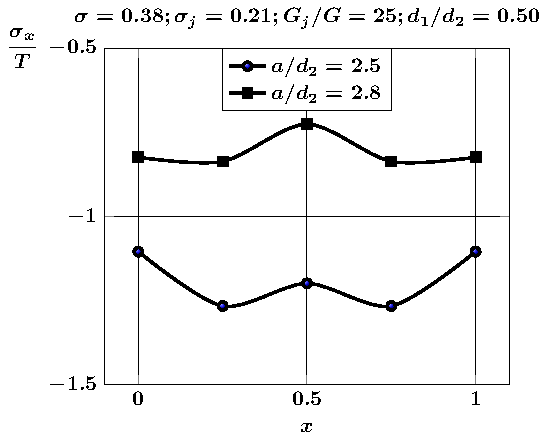
\includegraphics[width=7.8cm]{oblate-inc8-a-d50-g25-t1-sig_x.pdf}
\caption{Напряжения $\sigma_x/T$ на линии $AB$ в зависимости от расстояния между включениями при одноосном растяжении
\label{f:10:14}}}\hfil\hfil
\parbox[b]{7.5cm}{\centering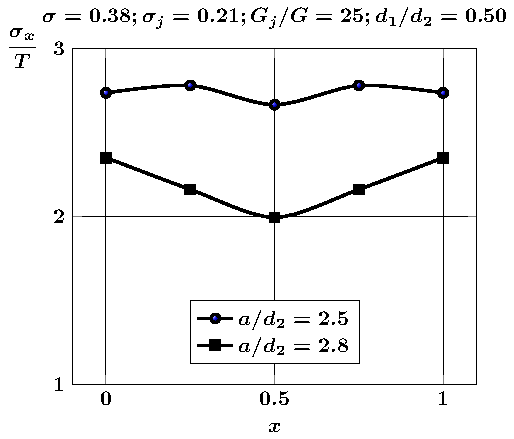
\includegraphics[width=7.5cm]{oblate-inc8-a-d50-g25-t2-sig_x.pdf}
\caption{Напряжения $\sigma_x/T$ на линии $AB$ в зависимости от расстояния между включениями при двуосном растяжении
\label{f:10:15}}}
\end{figure}

\begin{figure}[h!]
\centering\footnotesize
\parbox[b]{7.5cm}{\centering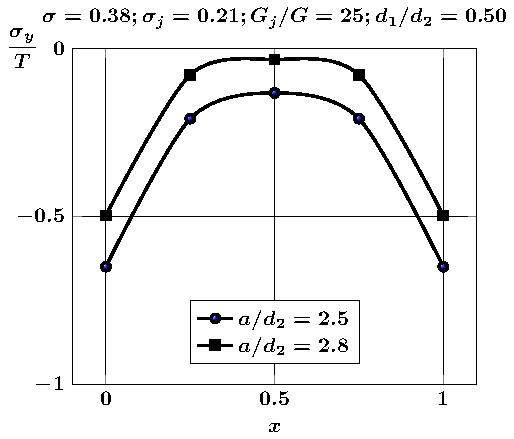
\includegraphics[width=7.6cm]{oblate-inc8-a-d50-g25-t1-sig_y.pdf}
\caption{Напряжения $\sigma_y/T$ на линии $AB$ в зависимости от расстояния между включениями при одноосном растяжении
\label{f:10:16}}}\hfil\hfil
\parbox[b]{7.5cm}{\centering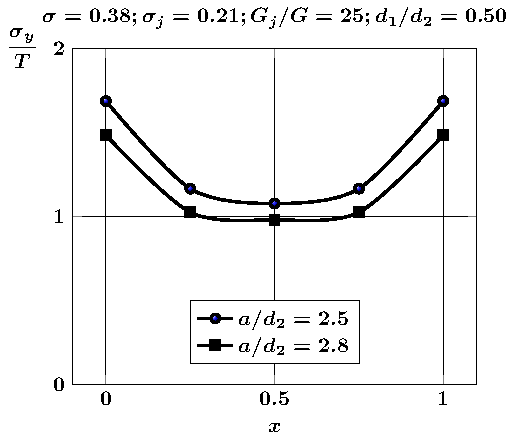
\includegraphics[width=7.6cm]{oblate-inc8-a-d50-g25-t2-sig_y.pdf}
\caption{Напряжения $\sigma_y/T$ на линии $AB$ в зависимости от расстояния между включениями при двуосном растяжении
\label{f:10:17}}}
\end{figure}

При численном анализе полагаем коэффициент Пуассона материала упругого пространства $\sigma=0.38$, а включения~--- $\sigma_j=0.21$, отношение модулей сдвига $G_j/G=25$. Включения считаем одного размера, отношение полуосей сфероидов $d_1/d_2=0.5$. Разрешающую систему уравнений численно решают методом редукции. На основании полученных решений находят нормальные напряжения на площадках, параллельных координатным плоскостям.

На рис.~\ref{f:10:14}~--- \ref{f:10:19} приведены напряжения $\sigma_x/T$, $\sigma_y/T$ и $\sigma_z/T$ на линии $AB$ (см.~рис.~\ref{f:10:1o}) при одноосном и двуосном растяжениях упругого пространства в зависимости от относительного расстояния $a/d_1$ между полостями.

\begin{figure}[h!]
\centering\footnotesize
\parbox[b]{7.5cm}{\centering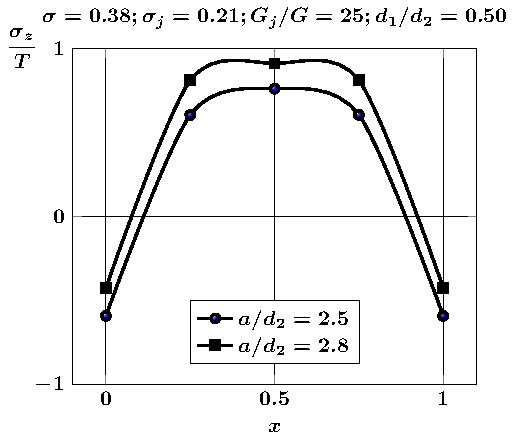
\includegraphics[width=7.6cm]{oblate-inc8-a-d50-g25-t1-sig_z.pdf}
\caption{Напряжения $\sigma_z/T$ на линии $AB$ в зависимости от расстояния между включениями при одноосном растяжении
\label{f:10:18}}}\hfil\hfil
\parbox[b]{7.5cm}{\centering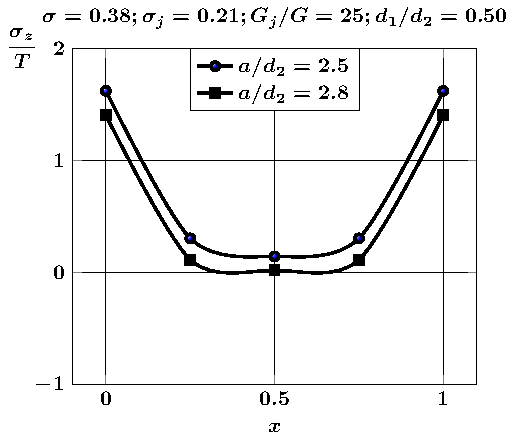
\includegraphics[width=7.6cm]{oblate-inc8-a-d50-g25-t2-sig_z.pdf}
\caption{Напряжения $\sigma_z/T$ на линии $AB$ в зависимости от расстояния между включениями при двуосном растяжении
\label{f:10:19}}}
\end{figure}


\end{russian}